\newpage
\section{NumPy, SciPy a matplotlib}
\subsection{numpy}
Tyto tři knihovny tvoří základ mnoha (pravděpodobně většiny) vědeckých skriptů v Pythonu. NumPy poskytuje pole numpy, rychlý způsob ukládání numerických dat v paměti, a funkce pro práci s nimi. SciPy poskytuje velké množství algoritmů včetně fitování metodou nejmenších čtverců, zpracování signálu nebo prostorového shlukování a matplotlib umožňuje vytváření vysoce kvalitních a přizpůsobitelných grafů. Obě jsou navrženy pro práci s poli numpy.

\begin{syntax}[Instalace balíčků -- pip]
    Balíčky, které nejsou standardně nainstalovány, lze nainstalovat pomocí nástroje příkazového řádku \ls{pip}, který stahuje balíčky registrované v Python Package Index (PyPI, \url{https://pypi.org/}). Například pro instalaci balíčku \ls{lmfit} spusťte v příkazovém řádku následující příkaz (funguje také v ipython REPL, např. ve Spyderu)
    \begin{lstlisting}
        pip install lmfit
    \end{lstlisting}
    Pro odstranění balíčku použijte \ls{uninstall} a pro upgrade \ls{install -U}. Spusťte \ls{pip help} pro úplný seznam dostupných příkazů. Pokud je vaše virtuální prostředí aktivováno, pip instaluje balíčky do tohoto virtuálního prostředí.

    Pokud používáte \ls{uv}, příkaz \ls{uv pip} je kompatibilní se standardním \ls{pip}, např. můžete použít \ls{uv pip install lmfit}. Nebo, pokud chcete svůj projekt zabalit pro použití jinými lidmi, můžete použít \ls{uv add lmfit}, což také přidá \ls{lmfit} jako závislost vašeho balíčku.
\end{syntax}

To use numpy we do
\begin{lstlisting}
    import numpy as np
\end{lstlisting}
there are several ways to create an array, e.g.
\begin{lstlisting}[caption=Tvorba polí.]
    #přímo ze seznamů
    arr = np.array([1,2,3,4])
    #2D pole
    arr_2D = np.array([[1,2,3],
                       [4,5,6],
                       [7,8,9]])
    # podobné list(range()), ale ani start, stop, ani step nemusí být celá čísla
    arr = np.arange(start, stop, step)
    #lineárně rozložené hodnoty
    arr = np.linspace(start, stop, count)
    #vyplněné nulami
    np.zeros(length)
    #vyplněné jedničkami
    np.ones(length)
\end{lstlisting}

Standardně pole np ukládají typ float. Pro jedničky a nuly je často užitečné použít booleovské hodnoty (True a False), jelikož \lstinline{np.ones(10, dtype=bool)} vytvoří pole o délce 10 vyplněné hodnotami True. Aritmetika funguje po prvcích, proto při sčítání/násobení/dělení/porovnávání musí mít pole stejnou délku, např.
\begin{lstlisting}
    >>> np.array([1,2,3]) + np.array([4,5,6])
    array([5,6,7])
\end{lstlisting}
Pokud je však jeden z operandů skalární číslo, operace se \emph{rozesílá} (broadcasts), např.
\begin{lstlisting}
    >>> np.array([1, 2, 3]) + 10
    array([11, 12, 13])
\end{lstlisting}

Řezání polí (slicing) funguje podobně jako řezání seznamů, např. \lstinline{arr[start:stop:step]}. Navíc můžeme také indexovat do pole pomocí seznamu indexů, např. \lstinline{arr[[0, 2, 4]]} vrátí pole obsahující 1., 3. a 5. prvek pole \lstinline{arr}. Nakonec, pomocí booleovských polí můžeme vytvořit podmnožinu prvků pole, kde je indexovací pole pravdivé, např.
\begin{lstlisting}
    arr1 = np.linspace(0, 10, 50)
    b = np.sqrt(arr1) > 3 # pole booleovských hodnot True, kde np.sqrt(arr1) > 3
    arr1[b] # pouze prvky arr1, jejichž druhá odmocnina je větší než 3
\end{lstlisting}

\begin{exercise}
    Napište program, který (ve smyčce) sečte čísla $1 + 2 + 3 + ... + n$ pro libovolné $n$ pomocí polí \verb|numpy| a porovná výsledek s Gaussovým vzorcem $n(n+1)/2$ pro uživatelem zadané $n$. \emph{Nápověda:} \verb|np.arange|
\end{exercise}
\begin{exercise}
    Napište funkci, která vrátí všechna prvočísla menší než $N$ pomocí metody Eratosthenova síta. \emph{Nápověda:} \verb|enumerate()|, \verb|np.ones(N, dtype=bool)|, maskování booleovským polem.
\end{exercise}

\subsubsection{Základní míry a operace s poli}
Jelikož jsou pole numpy určena především pro numerická data, mají v sobě zabudováno několik metod, které počítají některé základní míry, např.

\begin{tabular}{lll}
\ls{arr.mean()} & průměr pole\\
\ls{arr.std()} & směrodatná odchylka, vychýlený odhad rozptylu\\
\ls{arr.sum(), arr.cumsum()} & suma a kumulativní suma\\
\ls{arr.max(), arr.min()} & maximum a minimum\\
\ls{arr.argmax(), arr.argmin()} & index maxima a minima\\
\end{tabular}

Jako u každého kontejnerového typu vrací \ls{len(arr)} délku pole. Tyto metody existují také ve formě funkcí (např. můžeme volat \ls{np.mean(arr)}). Dále existují užitečné funkce, které pracují s poli v samotném modulu: \ls{np.diff(arr)} vrací pole rozdílů mezi nejbližšími sousedy o jeden prvek kratší než \ls{arr}; pro obecnější vážené průměrování lze použít \ls{np.average(arr, weights)}. Většina těchto funkcí má své odpovídající nan- verze, které ignorují hodnoty NaN v polích (např. \ls{np.nansum, np.nanmax} atd.). \ls{np.isnan(arr)} vrací pole stejné délky jako \ls{arr} s hodnotou True všude tam, kde \ls{arr} bylo NaN. Pro pole s booleovskými hodnotami jsou rozšířením \ls{and} a \ls{or} funkce \ls{np.logical_and(arr1, arr2)} a \ls{np.logical_or(arr1, arr2)} a podobně \ls{np.logical_not(arr)}, které vytvářejí nové pole s logickou operací aplikovanou na každý prvek vstupních polí. Logické operátory samy o sobě s poli nefungují.

\begin{syntax}[NaNs and Infs.]
     Matematické operace mohou vést buď k Not-a-Number (NaN) nebo nekonečnům, které jsou v numpy reprezentovány jako \ls{np.nan} a \ls{np.inf}. Jsou to speciální hodnoty indikující, pro NaN, že byla provedena nedefinovaná operace, např. \ls{np.log(-1)} (Python a Numpy podporují komplexní čísla, ale předpokládá se, že operace s reálnými čísly vedou také k reálným číslům -- pokud bychom chtěli použít komplexní logaritmus, museli bychom mu dát komplexní -1, tj. \ls{np.log(-1 + 0j)}).

    Jednoduché dělení nulou, např. 1/0, způsobí chybu ZeroDivisionError. Pokud je to však součástí \ls{np.array}, výsledkem bude $\pm$np.inf a varování (Warning), např. zkuste spustit \ls{np.array(1)/np.array(0)}.

    Myšlenka nehavarovat při nedefinovaných operacích nebo dělení nulou spočívá v tom, že často je poškozena pouze část pole (např. -1 může být zástupný symbol pro nedostupnou hodnotu) a může být jednodušší a čistší pokračovat za předpokladu, že všechny operace jsou platné, a na konci jednoduše vyhodit NaN hodnoty.
\end{syntax}

Pole lze seřadit na místě pomocí \ls{arr.sort()} nebo lze vytvořit nové seřazené pole pomocí \ls{sorted_arr = np.sort(arr)}. Pro získání pole indexů, které by pole seřadilo, můžeme použít \ls{np.argsort()}, což je užitečné, když chceme seřadit jedno pole podle druhého, např.
\begin{lstlisting}
    import numpy as np
    items = np.array(["Eggs", "Bread", "Apples"])
    prices = np.array([50, 20, 40])

    sort_ix = np.argsort(prices)
    print("Items sorted according to prices:")
    print(items[sort_ix]) # V českém kontextu: print(items[sort_ix])
\end{lstlisting}

\subsubsection{Vstup/výstup souborů}
Budeme používat numpy a matplotlib k analýze experimentálních dat. Nejprve musíme data získat, obvykle z nějakého souboru na disku. Za předpokladu, že máme data uložena jako textový soubor v \verb|data.txt| ve dvou sloupcích čísel oddělených tabulátory, můžeme je načíst do 2D pole numpy pomocí
\begin{lstlisting}
    arr = np.loadtxt("data.txt", comments='%', skiplines=3)
\end{lstlisting}
což načte \verb|data.txt| do 2D pole \verb|arr|, ignoruje všechny řádky začínající \% a přeskočí první tři datové řádky. Pokud jsou naše data oddělena čárkami (tj. soubor \verb|.csv|) místo tabulátorů, můžeme přidat klíčový argument \verb|delimiter=','| nebo použít \lstinline{np.genfromtxt(..., delimiter=',')}.

\begin{syntax}[Paths]
    Cesty k souborům nebo adresářům mohou být absolutní nebo relativní. Absolutní cesta specifikuje absolutní pozici souboru v souborovém systému, na Windows bude typicky začínat něčím jako \verb|C:\| a na Linuxu nebo Macu kořenovým adresářem \verb|/|.

    Relativní cesta je vztažena k aktuálnímu pracovnímu adresáři, který lze získat pomocí \ls{getcwd()} z modulu \ls{os}.

    Různé operační systémy používají různé oddělovače adresářů, tj. Windows používá \verb|\|, Linux a Mac \verb|/| a japonské počítače s Windows používají \verb|¥|. Pro spojení názvů adresářů způsobem, který bude fungovat všude, můžeme použít \ls{os.path.join('dir1', 'dir2', 'dir3', ...)}.

    Pro nalezení více souborů, jejichž název odpovídá vzoru, můžeme použít funkci \ls{glob()} z modulu \ls{glob()}. Například \ls{glob(os.path.join("photos", "photo*.png"))} vrátí seznam všech souborů, které odpovídají vzoru \ls{\"photos/photo<libovolný počet libovolných znaků>.png\"}.
\end{syntax}

Použití funkcí pro vstup/výstup souborů ze standardní knihovny Pythonu je také možné. Funkce \lstinline{file = open(filename, mode)} otevře soubor v daném režimu, nejběžnější jsou \lstinline{'r'} pro čtení, \lstinline{'w'} pro (pře)psaní a \lstinline{'a'} pro připojení. Veškerý obsah souboru lze přečíst najednou pomocí \lstinline{file.readlines()} nebo můžeme iterovat přes řádky souboru pomocí cyklu for (viz příklad níže). Inverzně existuje \lstinline{file.write(some_string)} (pokud je soubor otevřen v režimu 'r', toto selže). Zvláště pro zápis je důležité zavolat \lstinline{file.close()} poté, co jsme se souborem hotovi, jinak se změny nemusí zapsat na disk kvůli cachování.

Funkce \lstinline{np.loadtxt()} s výchozími argumenty je zhruba ekvivalentní
\begin{lstlisting}
    import numpy as np
    def my_load(fn):
        with open(fn, 'r') as file:
            rows = []
            for line in file:
                row = [float(s) for s in line.strip().split()]
                rows.append(row)
        return np.array(rows)
\end{lstlisting}
\begin{syntax}[with statement (basic)]
\lstinline{with} is an example of so-called context management which ensures that resources (in this case a file) are properly cleaned up after we are done using them. We will learn how to create our own context managers later, for now, the code
\lstinline{with} je příkladem tzv. správy kontextu, která zajišťuje, že zdroje (v tomto případě soubor) jsou po dokončení práce s nimi řádně uvolněny. Později se naučíme vytvářet vlastní správce kontextu, prozatím je kód
\begin{lstlisting}
    with open(fn, 'r') as file:
        do_stuff()
\end{lstlisting}
    zhruba ekvivalentní
\begin{lstlisting}
    file = open(fn, 'r')
    do_stuff()
    file.close()
\end{lstlisting}
s tou výhradou, že \ls{with} zajišťuje, že \lstinline{file.close()} se spustí, i když \lstinline{do_stuff()} způsobí pád programu.
\end{syntax}

\begin{exercise}
    Rozšiřte funkci \lstinline{my_load(fn)} z příkladu výše tak, aby podporovala komentáře v souborech.
\end{exercise}

\subsection{matplotlib}

matplotlib umožňuje vykreslování dat. Data vykreslujeme do os (axes), které jsou obsaženy v obrázcích (figures). Obrázek může obsahovat více os. Nejjednodušší způsob, jak vytvořit nový obrázek s novými osami, je \footnote{Všimněte si, že \lstinline{plt.subplots()} vrací dvě hodnoty. Vrací pouze jednu n-tici, která je destrukturována neboli rozbalena do dvou proměnných \lstinline{fig} a \lstinline{ax}.}
\begin{lstlisting}
    import matplotlib.pyplot as plt
    fig, ax = plt.subplots()
\end{lstlisting}
Pokud máme data v polích \lstinline{x} a \lstinline{y} stejné délky, můžeme je vykreslit například pomocí:
\begin{lstlisting}[caption=Základní vykreslování.]
    ax.plot(x, y, '-') # spojí dvojice bodů dané x a y plnými čarami
    ax.semilogy(x, y, '--s') # logaritmická osa y, čárkovaná čára se čtvercovými značkami
    ax.loglog(x, y, ':') # logaritmická osa x a y, tečkovaná čára
    ax.scatter(x, y) # bodový graf, nespojuje body čarami
\end{lstlisting}
Formát vykreslování je specifikován pomocí formátovacího řetězce bezprostředně za daty, který má formát \ls{fmt = [marker][line][color]}.\footnote{Viz \url{https://matplotlib.org/stable/api/_as_gen/matplotlib.pyplot.plot.html} pro úplný seznam možných formátů} Šířku čáry můžeme specifikovat pomocí klíčového slova \ls{lw=}, velikost značky pomocí \ls{ms=} a barvu pomocí \ls{color=} \footnote{Viz \url{https://matplotlib.org/stable/users/explain/colors/colors.html}} Všimněte si, že matplotlib nezajímá, zda dvojice polí x a y představuje matematickou funkci, jednoduše spojí body postupně čarami.

Pro popis os můžeme použít \ls{ax.set_xlabel()} a \ls{ax.set_ylabel()}. Data lze označit předáním klíčového argumentu \ls{label=} s řetězcem kterémukoli z vykreslovacích příkazů a následným zavoláním \ls{ax.legend()}. Obrázek můžeme uložit pomocí \ls{fig.savefig(filename)}.

Například pro vykreslení Gaussovy křivky s purpurovými čarami a azurovými body můžeme udělat
\begin{lstlisting}[caption=Kompletní příklad vykreslování.]
import numpy as np
import matplotlib.pyplot as plt

xs = np.linspace(0, 10, 100)
ys = np.exp(-(xs - 5)**2)

plt.close('all') #zavře všechny dosud otevřené obrázky
fig, ax = plt.subplots()

ax.plot(xs, ys, '--s', ms=5, lw=2, color='magenta', label=r'ax.plot($e^{-x^2}$)')
ax.scatter(xs, ys, s=ys*10, marker='o', color='cyan', zorder=3,
           label=r'ax.scatter($e^{-x^2}$)')

ax.set_xlabel('$x$ values')
ax.set_ylabel(r'the gaussian $e^{-(x-5)^2}$')
#kam umístit legendu, můžeme také použít "best" a nechat matplotlib hádat
ax.legend(loc='upper left')

fig.tight_layout() #redukuje některé bílé místo kolem okrajů
fig.savefig('gaussian.pdf') #formát souboru obrázku je odvozen z přípony
\end{lstlisting}
\begin{center}
    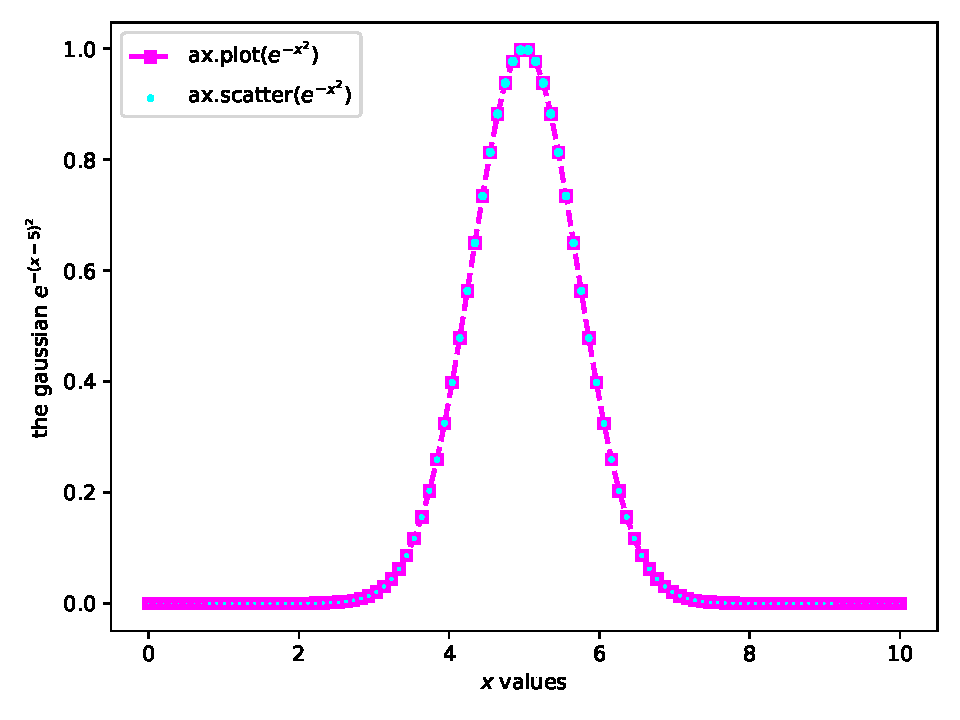
\includegraphics[width=0.5\linewidth]{gaussian.pdf}
\end{center}
Všimněte si, že můžeme ovládat, které objekty se kreslí nad kterými, pomocí klíčového argumentu \ls{zorder=} a že je podporována základní sazba matematiky \LaTeX, ale příkazy latexu začínající zpětným lomítkem je třeba buď escapovat (tj. \verb|"$\\frac{}{}$"|) nebo použít v raw řetězcích (tj. \verb|r"$\frac{}{}$"|).

\begin{exercise}
    Napište program, který pomocí NumPy a Matplotlib vykreslí výrazy $y=x$, $y=x^2$ a $y=\sqrt{x}$ od $x=0$ do $x=5$ s různými styly čar (např. plná, čárkovaná, tečkovaná) a uživatelem zadaným počtem bodů. Vyzkoušejte lineární, semilogaritmické a logaritmické osy. Popište osy a křivky.
\end{exercise}

Jeden obrázek může obsahovat více os vytvořených předáním volitelných argumentů rows a columns funkci \ls{plt.subplots()}. Více os je vytvořeno v pravidelné mřížce se zadaným počtem řádků a sloupců. Pro osy nerovných velikostí můžeme specifikovat poměry jejich šířek a výšek pomocí \ls{width_ratios} a \ls{height_ratios} (viz \ls{gridspec} \footnote{\url{https://matplotlib.org/3.5.0/tutorials/intermediate/gridspec.html}} pro složitější rozvržení obrázků). Osy mohou sdílet rozsahy x a y specifikováním booleovských klíčových argumentů \ls{sharex} a \ls{sharey}, například
\lstinputlisting[caption=Více os v jednom obrázku.]{../example_code/multiple_axes.py}
\begin{center}
    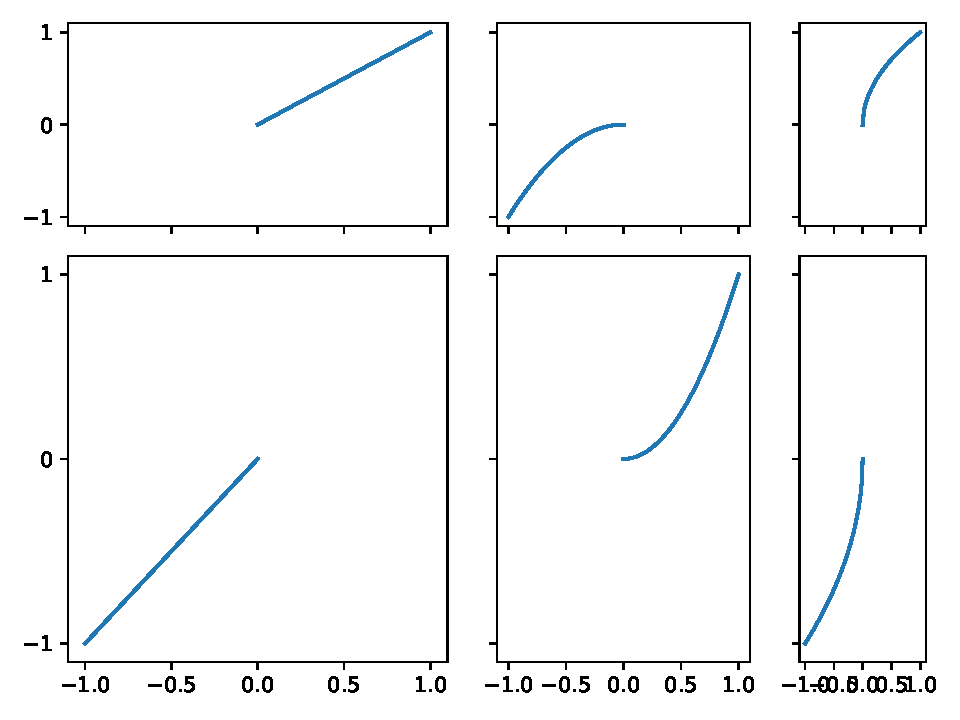
\includegraphics[width=0.5\linewidth]{multiax.pdf}
\end{center}
\begin{exercise}
    \label{ex:peak}
    Write a program that will read the data from "data.txt" which contains three columns of numbers separated by tabs. Let's call these columns frequency, $X$ and $Y$. Plot the frequency dependence of $X$ and $Y$ 
    \begin{enumerate}
        \item ve stejných osách ($X$ plná čára, $Y$ čárkovaná čára)
        \item v oddělených osách ve stejném obrázku se sdíleným rozsahem x a y
    \end{enumerate}
    Vykreslete také $X$ vs. $Y$ v samostatném grafu. Popište osy vhodně.
\end{exercise}
\begin{syntax}[Writing modules.]
    Jakýkoli python soubor může být importován jiným python souborem jako modul pomocí klíčového slova \ls{import}, název modulu je název souboru (bez koncovky .py). Při \ls{import}u je soubor nejprve spuštěn, tj. jakýkoli kód, který se nachází mimo definice funkcí, se spustí, například vezměme dva soubory ve stejném adresáři

    \verb|module.py|:
    \begin{lstlisting}
        def my_module_function(x):
            return 1 + x

        print("Ahoj moduly!")
    \end{lstlisting}

    \verb|module_user.py|:
    \begin{lstlisting}
        import module as m
        print(m.my_module_function(1))
    \end{lstlisting}

    Po spuštění \verb|module_user.py| se vytiskne "Ahoj moduly!". To obvykle není žádoucí. Abychom zabránili spuštění jakéhokoli kódu při importu a povolili jeho spuštění pouze tehdy, když je soubor spuštěn přímo, můžeme udělat
\begin{lstlisting}
    if __name__ == '__main__':
        print("Hello modules.")
\end{lstlisting}
    Here, \ls{__name__} is a special variable defined by Python itself that contains the name of the module associated with the current file. Its value is \ls{'__main__'} if and only if it was directly.

    Aby bylo možné soubor importovat jako modul, Python ho musí být schopen najít. Standardně Python hledá v aktuálním pracovním adresáři \ls{os.getcwd()} a v adresářích uvedených v seznamu \ls{sys.path} v balíčku \ls{sys}. Pokud chceme načíst balíček odjinud, můžeme jednoduše přidat jeho adresář do proměnné path pomocí \ls{sys.path.append()}.
\end{syntax}
\begin{exercise}
    \label{ex:peaks}
    Najděte maximum a minimum absolutní hodnoty $R = \sqrt{X^2 + Y^2}$ a vyznačte jejich pozice svislými čarami v grafu frekvenční závislosti $X$ a $Y$ z předchozího cvičení. Odhadněte plnou šířku v polovině maxima (FWHM) píku a činitel jakosti $f_0$/FWHM, kde $f_0$ je frekvence maximální odezvy. 
    
    \emph{Hint:} \ls{np.argmin, np.argmax}, \ls{ax.axvline, ax.axhline}
\end{exercise}
\begin{exercise}
    \label{ex:peaks-all}
    Zpracujte všechny soubory z adresáře \ls{lots_of_data} podobně jako v Cvič.~\ref{ex:peaks}. Vykreslete FWHM jako funkci $f_0$. Použijte řešení Cvič.~\ref{ex:peaks} jako modul.
    
    \emph{Hint:} \ls{glob}
\end{exercise}

Veličiny, které závisí na dvou řídicích proměnných, lze často vykreslit pomocí teplotních map (heat maps), pro které můžeme použít \ls{ax.imshow(arr2D)}, která vezme 2D pole čísel a mapuje je na barvu pixelu pomocí barevné mapy (colormap)\footnote{Viz \url{https://matplotlib.org/stable/users/explain/colors/colormaps.html} pro úplný seznam názvů barevných map.} Všimněte si však, že \ls{imshow()} se primárně používá pro obrázky, které konvenčně začínají v levém horním rohu s levotočivými osami. Data typicky začínají v levém dolním rohu s pravotočivými osami. To lze změnit specifikováním klíčového slova \ls{origin='lower'} pro \ls{imshow()}. Alternativně, pro vykreslování dat, která nejsou na pravidelné mřížce, můžeme použít \ls{ax.pcolormesh(X, Y, Z)}, kde \ls{X, Y, Z} jsou 2D pole.

Například pro vykreslení 2D Gaussovy křivky s barevnou mapou \ls{'inferno_r'},
\begin{lstlisting}[caption=Příklad dvourozměrného vykreslování.]
import numpy as np
import matplotlib.pyplot as plt

#x and y axis
_xs = np.linspace(0, 10, 100)
_ys = np.linspace(0, 10, 100)
#but we need 100 x 100 points for both x and y that sample the 
#celý interval (0, 10) x (0, 10), to lze provést pomocí
#meshgrid
xs, ys = np.meshgrid(_xs, _ys)
zs = np.exp(-(xs - 5)**2 - (ys - 5)**2)

plt.close('all') #zavře všechny dosud otevřené obrázky
fig, ax = plt.subplots()

plot = ax.imshow(zs, cmap='inferno_r', origin='lower')
#podobně
#plot = ax.pcolormesh(xs, ys, zs, cmap='inferno_r') 
cbar = fig.colorbar(plot) #the color axis scaling
cbar.set_label('$z$')
ax.set_xlabel('$x$')
ax.set_ylabel('$y$')
\end{lstlisting}
\begin{center}
    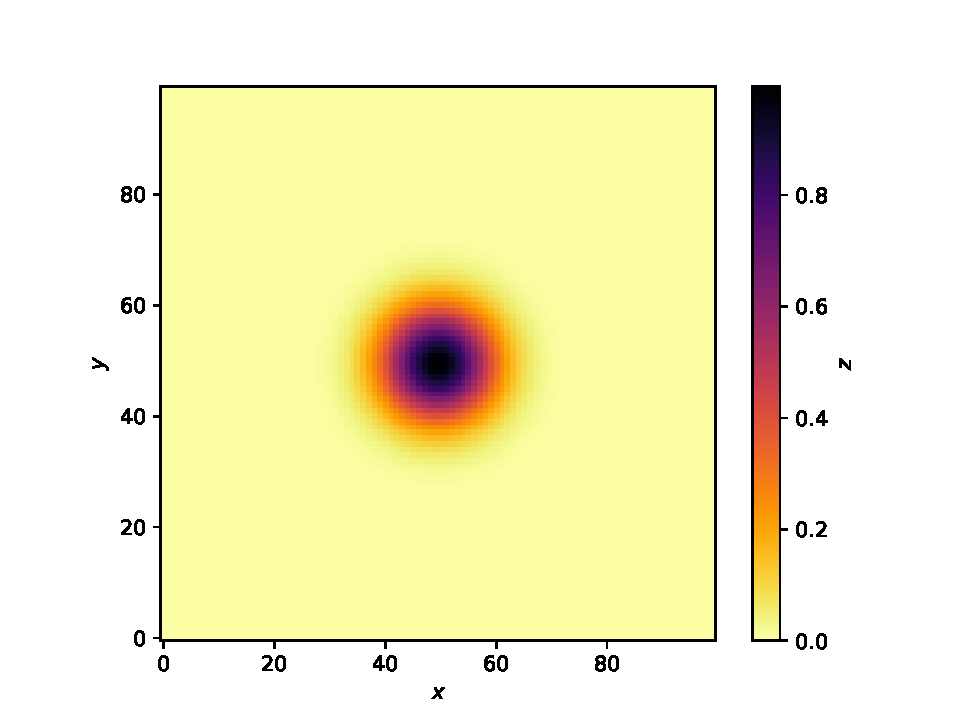
\includegraphics[width=0.5\linewidth]{gaussian_2D.pdf}
\end{center}
\begin{exercise}
    Vykreslete Mandelbrotovu množinu s konfigurovatelným rozsahem a rozlišením.

    \emph{Nápověda:} Mandelbrotova množina je množina komplexních čísel $c$, pro která řada $z_{n+1} = z_n^2 + c,\; z_0 = 0$ nediverguje. Pokud $|z_n| \geq 2$ pro jakékoli $n$, řada bude divergovat. Jako kritérium konvergence můžeme použít, že $|z_n| < 2\; \forall n < N_\mathrm{max}$ ($N_\mathrm{max} = 100$, například). Vykreslete množinu pomocí \ls{plt.imshow(c)}, kde \ls{c[i,j]} je počet iterací potřebných k překročení $|z_n| = 2$ (nebo $N_\mathrm{max}$). Celá množina je obsažena v obdélníku s levým dolním rohem $-2-i$ a pravým horním rohem $1+i$ v komplexní rovině.
\end{exercise}

\subsubsection{Přehled základních příkazů pro vykreslování}
Za předpokladu, že obrázek a osy byly vytvořeny jako \ls{fig, ax = plt.subplots()}, základní příkazy pro manipulaci s grafem jsou

\begin{tabular}{p{40mm}p{100mm}}
     \ls{ax.xlabel("popisek x"), ax.ylabel("popisek y")} & nastaví popisky os \\
     \ls{ax.set_xlim(xmin, xmax), ax.set_ylim(ymin, ymax)} & nastaví limity os, xmin, xmax atd. lze také použít jako klíčová slova \\
     \ls{ax.set_aspect('equal')} & nastaví poměr stran os na stejný, užitečné, když obě osy obsahují kvalitativně podobná data\\
     \ls{ax.legend(loc=location)} & zobrazí legendu na místě \ls{location} $\in$ \ls{\"upper|lower left|right\"} nebo \ls{\"best\"} \\
     \ls{fig.tight_layout()} & upraví velikost os tak, aby se vešly všechny popisky a zmenšil se bílý prostor\\
     \ls{fig.supxlabel('xlabel'), fig.supylabel('ylabel')} & nastaví společné popisky os pro celý obrázek s více osami\\
     \ls{fig.colorbar()} & vytvoří barevnou škálu v obrázku\\
     \ls{plt.close('all')} & zavře všechny otevřené obrázky
\end{tabular}